\section{Methode nach Stam}
\label{sec:stam}

\subsection{Fluiddynamik in interaktiven Anwendungen}

Numerische Strömungsmechanik (\Pimiddyengl{}\PimiddyEnglBegriff{computational
fluid dynamics} oder CFD) war ursprünglich ein Problem, das nur mit
leistungsfähigen Rechenclustern angegangen werden konnte. Diese
benötigten mehrere Minuten bis mehrere Tage, um ein Ergebnis zu
liefern.

Deshalb wurden Probleme, die auf CFD zurückzuführen sind (wie die
Simulation von Rauch, Wolken oder eben Wind) nicht physikalisch
modelliert, sondern nur visuell
angenähert. \cite{Sims:1990:PAR:97880.97923} beschreibt beispielsweise
ein Partikelsystem, bei dem die Partikel sich um
\PimiddyQuotes{Wirbelpunkte} bewegen, die entweder zufällig generiert
oder vom Designer erstellt wurden. Dadurch werden die ansonsten schwer
zu berechnenden Geschwindigkeitsfelder approximiert. Mit Hilfe dieser
Technik entstand der Film \PimiddyQuotes{Particle
Dreams} (\cite{ParticleDreams}), in dem auch ein Schneesturm modelliert
wurde.

Ein erstes auf die Computergrafik angepasstes, physikalisches Modell,
stellten \PimiddyName{Foster} und \PimiddyName{Metaxas} 1997 in \cite{Foster1997} vor. Es war
allerdings numerisch nicht stabil und daher schlecht für
Echtzeitanwendungen geeignet. Ein Simulationsschritt benötigte damals
außerdem noch \Pimiddyca{} 15 Sekunden zur Berechnung. 1999 erschien \PimiddyName{Stams}
wegweisendes Paper \PimiddyQuotes{Stable Fluids} (\cite{Stam1999}),
welches zum ersten Mal ein numerisch stabiles Verfahren enthielt
(daher \PimiddyQuotes{stable}), das (nach eigenen Angaben)
Echtzeitsimulationen ermöglicht, wenn auch nur für zweidimensionale
Felder. Das Verfahren wird im Folgenden mit SF abgekürzt.

Etwa zur gleichen Zeit wurden zwei weitere Ansätze für die schnelle
Simulation von Strömungen entwickelt, die wegen ihrer Komplexität hier
nicht weiter vertieft werden sollen:
\begin{itemize}
\item Basierend auf zellulären Automaten wurde das
\PimiddyBegriff{Lattice-Bolzmann-Verfahren} (LBM) für die Simulation
eingesetzt, welches --- ähnlich Stams Ansatz --- datenparallel
formuliert ist und komplexe Hindernisse innerhalb der Simulation
zulässt. Es wird sowohl für Gase als auch für Flüssigkeiten
eingesetzt (\cite{Chen1998}).
\item Basierend auf Partikelsystemen wurde das ursprünglich in der
Astronomie entwickelte Verfahren \PimiddyBegriff{Smoothed Particle
Hydrodynamics} (SPH) vor allem für die Simulation von Flüssigkeiten
eingesetzt (\cite{Muller2003}).
\end{itemize}
Im Jahr 2003 übertrugen \PimiddyName{Krüger \Pimiddyetal}in
\cite{Kruger2005} einige algebraische Operatoren auf die GPU und
nutzten sie unter anderem, um SF auf der GPU umzusetzen, allerdings
vorerst nur im Zweidimensionalen. Sie erreichten bei einem Feld der
Größe $1024 \times 1024$ Wiederholraten von etwa 9 Bildern pro
Sekunde. Im selben Jahr implementierten \PimiddyName{Harris \Pimiddyetal}das Verfahren
auf der GPU im Dreidimensionalen und erreichten bei einem Feld der
Größe $32^3$ schon Wiederholraten um 27 Bilder pro
Sekunde. Strömungsmechanik in Echtzeit war zu diesem Zeitpunkt also
auf Desktop-PCs möglich.

Die GPU-Implementierungen nutzten allerdings die
Hardware-Grafikpipeline, die in \cref{sec:opengl} näher beschrieben
wird. Statt Daten aus Arrays einzulesen und mittels einer universellen
Programmiersprache wie C zu verarbeiten, waren von der Hardware einige
Einschränkungen vorgegeben. Als Datenstruktur standen beispielsweise
nur zweidimensionale Texturen zur Verfügung. Die Berechnungen mussten
zudem in einer Shadersprache wie GLSL verfasst werden, in der
Anweisungen zum Kontrollfluss wie \PimiddyzB{} Schleifen oft nur
eingeschränkt benutzbar waren. Das Spiel \PimiddyQuotes{Hellgate:
London} nutzte so erstmals die GPU, um dynamisch Rauch zu simulieren
und zu visualisieren (\cite{Crane2007}).

Die Grafikhardware entwickelte sich allerdings schnell und konnte
immer komplexere Berechnungen durchführen. Um allgemeine (also nicht
unbedingt grafikbezogene) Berechnungen aktiv zu unterstützen,
veröffentlichte NVidia 2006 die erste Version des CUDA-Frameworks. Mit
CUDA kann reiner C++-Code mit Abschnitten versehen werden, die dann
auf der Grafikkarte ausgeführt werden. Ein Jahr später veröffentlichte
\PimiddyName{Goodnight} eine Implementierung von SF mit Hilfe von
CUDA (\cite{Goodnight2007}).

CUDA-Programme laufen allerdings nur auf NVidia-Grafikkarten. Andere
Hersteller wie AMD veröffentlichten ihrerseits Frameworks für die
eigene Hardware. Es existierte jedoch kein übergreifendes System, bis Ende
2008 die erste OpenCL-Spezifikation veröffentlicht wurde. Viele
Hersteller implementierten daraufhin diesen Standard und
GPU-Programmierung wurde hardwareübergreifend.

Bislang sind allerdings noch keine Echtzeitanwendungen bekannt, die
Stams Verfahren oder OpenCL für die Berechnung von Windfeldern
nutzen. Daher soll in dieser Arbeit OpenCL genutzt werden, um SF auf
der GPU zu implementieren und das resultierende Windfeld für die
Bewegung der Schneeflocken zu verwenden.

\subsection{Motivation}

Die Methode zur approximativen Lösung der Navier-Stokes-Gleichungen,
die im Folgenden erklärt wird, wurde von \PimiddyName{Jos Stam} im
Jahr 1999 entwickelt und in dem Paper \PimiddyQuotes{Stable Fluids}
vorgestellt (\cite{Stam1999}). Das Verfahren wurde speziell für die
Computergrafik entwickelt, wobei auf einige Besonderheiten eingegangen
wurde:

\begin{enumerate}
\item
Im Gegensatz zu wissenschaftlichen Simulationen ist man in der
Computergrafik an einer Lösung interessiert, die in möglichst kurzen
Abständen Ergebnisse produziert. Um eine flüssige Simulation zu
erhalten, ist die Laufzeit des Lösungsalgorithmus auf 16 Millisekunden
(für 60 Bilder pro Sekunde) \Pimiddybzw{} 33 Millisekunden (für 30
Bilder pro Sekunde) beschränkt. Die Navier-Stokes-Gleichungen bilden
als System von nichtlinearen Differentialgleichungen hier eine
besondere Herausforderung.
\item
Bisherige Ansätze zur Strömungsmechanik kamen aus einem
wissenschaftlichen Bereich, in dem Exaktheit eine große Rolle
spielte. In der Computergrafik allgemein und auch bei der
Aufgabenstellung dieser Arbeit ist man allerdings nicht unbedingt an
einer exakten Lösung interessiert.  Ein physikalisch annähernd
korrektes Ergebnis genügt.
\item
Bisherige Verfahren (wie \PimiddyzB{} die finiten Differenzen in
\cite{Foster1997}) waren numerisch \emph{instabil} für große
Zeitschritte. Das bedeutet, die Simulation kann immer nur einen
bestimmten, kleinen Zeitabschnitt $\delta$ voranschreiten.
Echtzeitanwendungen wie Spiele oder Animationssoftware können
allerdings keine minimale Bildwiederholrate garantieren, da sie mit
verschiedenen Umgebungen und Hardwarekonfigurationen ausgeführt werden
können. Man hat im Allgemeinen also eine Simulationsschrittweite von
$\Delta$ gegeben, die auch größer sein kann als $\delta$.

Als Ausweg muss man einen großen Zeitschritt entweder ignorieren ---
was die Simulation unrealistisch macht --- oder ihn in
$\PimiddyAufrunden{\Delta / \delta}$ kleinere Zeitschritte
unterteilen. Die Zeit, die benötigt wird, um die Simulation ein
$\delta$ weiterzubewegen, ist aber konstant. Dies führt dazu, dass das
nächste Frame erneut viel Rechenzeit benötigt und wieder entsprechend
lang wird.

Dieser Effekt ist eventuell nicht mehr aufzuhalten, was eine
\PimiddyQuotes{Explosion} der Simulation zur Folge hat.
\item Bisherige approximative Verfahren waren auf Hilfe des Designers
angewiesen, um Teile der Simulation möglichst realistisch zu
modellieren. Bestimmte natürlich vorkommende Turbulenzen mussten
explizit in die Simulation eingegeben werden. Idealerweise sollte die
Simulation allerdings von selber fortgeführt werden, der Designer
sollte nur Rahmenbedingungen wie Hindernisse und globale Eigenschaften
des Fluids (wie Dichte und Viskosität) vorgeben.
\end{enumerate}

SF ist also auf Geschwindigkeit ausgelegt, basiert aber
nichtsdestotrotz auf den Navier-Stokes-Gleichungen und erzielt
akkurate Simulationsergebnisse. Anfängliche Schwachstellen des
Verfahrens, wie die zu starke Dämpfung von Wirbeln, wurden in weiteren
Arbeiten ausgebessert (\cite{Foster}). Diese Verbesserungen sind
teilweise in diese Arbeit eingeflossen.

Wegen der numerischen Stabilität und sehr guten Parallelisierbarkeit
wird Stams Verfahren bereits in einigen Spielen eingesetzt (siehe
\cite{Crane2007, Peschel2009}). Hier wird eine leicht abgewandelte
Fassung beschrieben, bei der andere Randbedingungen verwendet werden.

\subsection{Überblick über das Verfahren}

In diesem Abschnitt wird ein grober Überblick über die Bestandteile
des Verfahrens gegeben, die sich direkt aus den
Navier-Stokes-Gleichungen ergeben. Es werden außerdem die
Rahmenbedingungen erläutert.

Die Fluidsimulation findet auf einem endlichen Gitter, also einer
Teilmenge von $\PimiddyGanz^n$ statt. Gegeben sei das
Geschwindigkeitsfeld zum Zeitpunkt $t$:
$\vec{u}^{\PimiddyFormelText{ }t}$. Als Anfangszustand
könnten zum Zeitpunkt $t=0$ \PimiddyzB{} alle Zellen auf eine vorgegebene
\PimiddyQuotes{Windrichtung} gesetzt sein.  Gegeben sei außerdem ein
Zeitdelta $\Delta t$ (nicht zu verwechseln mit dem
Laplaceoperator). Ziel ist es, unter Zuhilfenahme der
Navier-Stokes-Gleichungen ein neues Geschwindigkeitsfeld
$\vec{u}^{\PimiddyFormelText{ }t+\Delta t}$ zu berechnen.

Außerdem berechnet man einmalig ein \emph{Hindernisfeld}
$b$. Ist $b_{i,j,k} = 1$, dann ist diese Zelle mit einem
Hindernis ausgefüllt. Ist $b_{i,j,k} = 0$, ist die Zelle frei. In
\cref{sec:implementation_boundaries} wird erklärt, wie dieses
Hindernisfeld gefüllt wird.

Die rechte Seite der \cref{eq:navier_stokes_momentum_equation} besteht
aus mehreren Summanden:

\begin{equation}
\vec{u} \PimiddyDiv \vec{u} -
\nu \PimiddyLaplace \vec{u} +
\vec{g} -
\frac{
	1
}
{
	\rho
}
\PimiddyGrad p
\end{equation}

In Stams Verfahren wird jeder dieser Summanden als eine Operation betrachtet,
die ein Geschwindigkeitsfeld sowie eventuell weitere Eingabegrößen wie $\Delta
t$ erhält, und die ein neues Geschwindigkeitsfeld zurückgibt. Das so berechnete
neue Feld wird zur Eingabe der darauffolgenden Operation verwendet. So
wird die Lösung der Impulsgleichung in kleinere Teile zerlegt, die für
sich behandelt werden können:

\begin{itemize}
\item
	Der Term
	\begin{equation}
	\vec{u} \PimiddyDiv \vec{u}
	\end{equation}
	stellt die \PimiddyBegriff{Advektion} dar. Das Vektorfeld wird entlang
	seiner eigenen Strömungsrichtung weiterbewegt. Sie sei im Folgenden mit
	\PimiddyInlineCode{advection}$(\vec{u},\Delta t)$ bezeichnet.
\item
	Der Term
	\begin{equation}
	\nu \PimiddyLaplace \vec{u}
	\end{equation}
	stellt die viskose \PimiddyBegriff{Diffusion} dar. Selbst wenn keine
	Kräfte auf das Fluid wirken, bewegt es sich durch Diffusionsprozesse
	weiter, so wie Farbe auf einem Blatt Papier verläuft.

	Dieser Term kann in SF ignoriert werden. Diffusion entsteht
	ohnehin \PimiddyQuotes{zufällig} durch Genauigkeitsfehler während der
	Advektion (siehe unten). Durchdas Vernachlässigen kann die
Performance erhöht werden, denn die Lösung dieses Terms ist sehr
aufwändig.
\item
	Der Term $\vec{g}$ umfasst schlicht die Summe aller äußeren
	Kräfte, die auf das Fluid wirken. Hierzu gehört sowohl die Schwerkraft
	als auch der von außen eingeführte Wind. Die Operation bekommt als
	Eingabe das Geschwindigkeitsfeld sowie das Zeitdelta (bei größerem
	Zeitunterschied zum letzten Simulationsschritt sollen die Kräfte
	stärker wirken). Sie sei im Folgenden mit
	\PimiddyInlineCode{externalForces}$(\vec{u},\Delta t)$ bezeichnet.
\item
	Der \emph{Druck} des Fluids wird in dem Term
	\begin{equation}
	-\frac{1}{\rho} \PimiddyGrad p
	\end{equation}
	zusammengefasst ($\rho$ bezeichnet die Dichte des Fluids). Er
        dient am Ende unter anderem dazu, die Randbedingungen und die
        Un"-komp"-ri"-mier"-bar"-keit zu erzwingen. Die Berechnung des
        Druckfeldes $p$ aus dem Geschwindigkeitsfeld $u$ sei mit
        \PimiddyInlineCode{calcPressure}$(\vec{u})$ bezeichnet.
\item
	Wie bei Differentialgleichungen üblich, müssen wir noch die
	\emph{Rand- und Anfangsbedingungen} behandeln. Dadurch wird
	einerseits sichergestellt, dass das Fluid nicht in Hindernisse
	eindringt und andererseits an den Rändern der Simulation frei hinausfließen
	kann. Diese Operation wird im Folgenden als
	\PimiddyInlineCode{boundaries}$(\vec{u})$ bezeichnet und wird noch vor der
	Berechnung des Drucks durchgeführt.
\end{itemize}

\begin{algorithm}
\caption{Der Lösungsalgorithmus in Pseudocode}
\label{alg:stam_first_algorithm}
\begin{algorithmic}
\Function{simulate}{$\vec{u}$,$\Delta t$}
	\State $\vec{u}'$ = advection($\vec{u}$,$\Delta t$)
	\State $\vec{u}''$ = externalForces($\vec{u}'$,$\Delta t$)
	\State $\vec{u}'''$ = boundaries($\vec{u}''$)
	\State $p$ = calcPressure($\vec{u}$)
	\State \Return $\vec{u}''' - \PimiddyGrad p$
\EndFunction
\end{algorithmic}
\end{algorithm}

\begin{figure}[h]
\centering
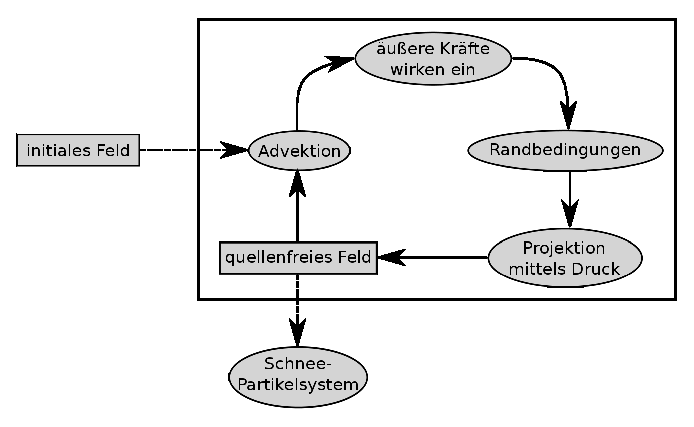
\includegraphics[width=12cm]{images/stam_loop_with_projection}
\caption{Die Simulationsschleife. Projektion bezeichnet die Berechnung des Druckgradienten und die Subtraktion des Gradienten vom Geschwindigkeitsfeld. Es entsteht ein quellenfreies Vektorfeld, welches wieder in den Advektionsalgorithmus gespeist werden kann. Dieses Feld wird zudem für die Beeinflussung der Schneepartikel verwendet.}
\label{fig:stam_loop_with_projection}
\end{figure}

Für jede Operation wird im Folgenden ein Lösungsalgorithmus
vorgestellt, insgesamt erhält man aus der Impulsgleichung den Pseudocode in
\cref{alg:stam_first_algorithm}. Eine grafische Darstellung findet
sich in \cref{fig:stam_loop_with_projection}.

\subsection{Advektion}
\label{sec:stam_advection}

Wie bereits in der Erklärung der Navier-Stokes-Gleichungen angedeutet, wird bei
der Advektion das Geschwindigkeitsfeld entlang \PimiddyQuotes{sich selber}
weiterbewegt. Auf diese Weise kann sich Wind, der von einer Seite der
Simulation eingeführt wird, über den gesamten Simulationsbereich ausbreiten.
Manchmal spricht man auch von \emph{Selbstadvektion}. In älterer Literatur
ist auch von \emph{Konvektion} die Rede.

Im Folgenden gehen wir etwas allgemeiner davon aus, dass eine
\emph{beliebige} Größe $q_{i,j,k}^{t}$ entlang des Vektorfelds
$\vec{u}$ bewegt werden soll. Die Methode
\PimiddyInlineCode{advection}$(q,\Delta t)$ kann also auch verwendet
werden, um Temperaturwerte oder die Dichte des Rauchs an einer Stelle
entlang des Vektorfelds weiterzubewegen. Als Ausgabe erhalten wir ein
neues Feld $q^{t+\Delta t}$.

Um die Advektion durchzuführen gibt es mehrere Ansätze. Der gängigste
arbeitet mit der Methode der finiten Differenzen und wurde unter
anderem in~\cite{Foster} benutzt. Finite Differenzen führen allerdings
zu einem numerisch instabilen Algorithmus, wie in der Einleitung
bereits erwähnt. Daher wird eine andere Vorgehensweise gewählt. Ein
ebenfalls numerisch instabiler Ansatz wird leicht modifiziert, um
Stabilität zu erreichen und ihn ohne Einschränkungen verwenden zu
können.

\begin{figure}[h]
\centering
%\def\svgwidth{\textwidth}
%\input{images/advection_bad.eps_tex}
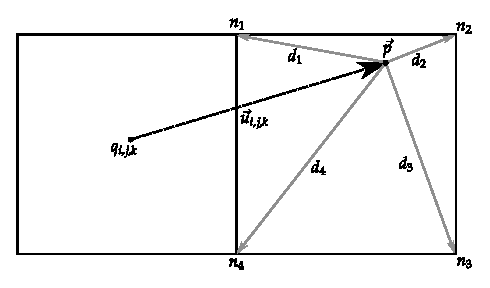
\includegraphics[width=12cm]{images/advection_bad}
\caption{Das numerisch instabile Advektionsverfahren}
\label{fig:stam_numerically_unstable_advection}
\end{figure}

Das zu berechnende neue Feld $q^{t+\Delta t}$ sei anfangs
überall 0 (\Pimiddybzw{} $(0,0,0)$, falls es ein Vektorfeld ist). Man stelle
sich nun an jedem Gitterpunkt $(i,j,k)$ ein Partikel mit
\PimiddyQuotes{Ladung} $q_{i,j,k}$ vor, welches im Fluid treibt. Das
Partikel wird durch das Fluid beschleunigt und dadurch um $\Delta t
\cdot \vec{u}_{i,j,k}$ verschoben. Es befindet sich im nächsten
Zeitschritt bei
\begin{equation}
\vec{p}=(i,j,k)+\Delta t \cdot \vec{u}_{i,j,k}
\end{equation}

Somit liegt es im Allgemeinen nicht mehr \emph{exakt} auf einem
Gitterpunkt, sondern zwischen 8 Nachbarpunkten $n_i \in
\PimiddyGanz^3, i \in \{1,\ldots,8\}$ (siehe
\cref{fig:stam_numerically_unstable_advection}). Zu jedem dieser
Nachbarpunkte kann man den Abstand $d_i$ zum Partikel bestimmen:

\begin{equation}
d_i = \PimiddyNorm{2}{\vec{p} - n_i}, i \in \{1,\ldots,8\}
\end{equation}

Diese $d_i$ dienen als Gewichtung, um die \PimiddyQuotes{Ladung} $q_{i,j,k}$
anteilig auf die Nachbarknoten aufzuteilen:

\begin{equation}
q_{n_i}' \leftarrow q_{n_i}' + d_i \cdot q_{i,j,k}
\end{equation}

Dieses Verfahren ist intuitiv und einfach zu implementieren. Aber es ist
numerisch nicht stabil und führt zu Oszillationen.

Stam wählte einen anderen Ansatz, die sogenannte \emph{Methode der
Charakteristika}. Die Idee ist ähnlich zu der gerade vorgestellten, funktioniert
aber in die \PimiddyQuotes{umgekehrte Richtung}.

\begin{figure}[ht]
\centering
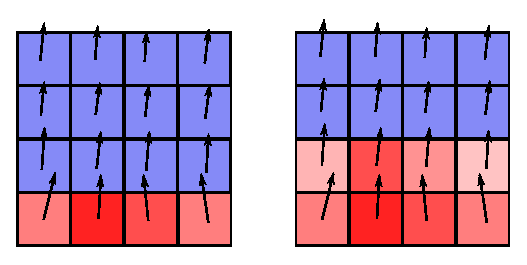
\includegraphics[width=12cm]{images/advection_bad_example}
\caption{Ein Schritt des numerisch instabilen Advektionsverfahrens, angewendet auf ein Temperaturfeld. Die roten Werte deuten eine Temperaturquelle an. Der anfänglich kalte Raum erwärmt sich durch das Verfahren langsam.}
\end{figure}

Man betrachtet wieder jeden Gitterpunkt $(i,j,k)$ einzeln, stellt sich
diesmal allerdings vor, man sei auf der Zeitachse im Punkt $t+\Delta
t$, also bereits im nächsten Zeitschritt. Das gedachte Partikel an
Position $(i,j,k)$ habe die Geschwindigkeit
$\vec{u}_{i,j,k}^{\PimiddyFormelText{ }t}$.

Rechnet man auf der Zeitachse um $\Delta t$ zurück, erhält man die
\PimiddyQuotes{vorherige} Position des Partikels, nämlich $(i,j,k) -
\Delta t \cdot \vec{u}_{i,j,k}^{\PimiddyFormelText{ }t}$. Es ergibt
sich dasselbe Problem wie bei dem vorher beschriebenen Ansatz: Die
Position liegt nicht genau auf dem Gitter, sondern dazwischen (siehe
\cref{fig:stam_good_advection})\PimiddyFootnote{Hier wird nur ein
Schritt der Partikelflugbahn zurückverfolgt. Es besteht die
Möglichkeit, mehrere Schritte zurückzuverfolgen, die aber
aufwändiger zu implementieren ist.}.

Als Lösung \emph{interpolieren} wir zwischen den 8 Nachbarwerten des
verschobenen Partikels und schreiben den resultierenden Wert in die Zelle
$\vec{u}_{i,j,k}^{\PimiddyFormelText{ }t+\Delta t}$. Dies ist eine Operation, auf die Grafikkarten stark
optimiert sind, und bei denen Texturen hohe Performance erreichen
können.

Allerdings liegt hier auch eine Fehlerquelle des Verfahrens. Interpolation ist
eine glättende Operation, sie liefert nur eine \emph{Approximation} des Wertes,
der zwischen den Gitterzellen angenommen würde. Ähnlich wie bei der
Herleitung der diskreten Ableitung in \cref{sec:mathematics_discretization}
muss man in der Implementierung einen Kompromiss eingehen und ein
Interpolationsverfahren wählen, welches Genauigkeit und Rechenleistung verbindet.

Auch für große Zeitschritte liefert das Verfahren ein Vektorfeld,
welches in seinem Wertebereich beschränkt ist, denn die Interpolation liefert nie einen
Wert zurück, der betragsmäßig größer ist als die Ausgangswerte. Das Verfahren
ist deshalb stabil.

Allerdings sollte $\Delta t$ nicht zu groß gewählt werden.
\cite{Foster} gibt hier als Richtlinie etwa $5\times$ die Gittergröße
an. Diese Art der Advektion wird auch
\PimiddyBegriff{semilagrange'sche Advektion} genannt, da zwar ein
diskretes Gitter verwendet wird, aber die Flugbahn von Partikeln das
Verfahren motiviert.

\begin{figure}[ht]
\centering
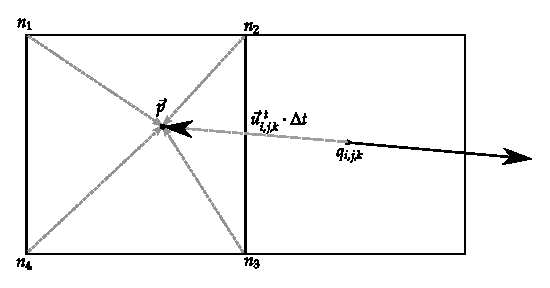
\includegraphics[width=12cm]{images/advection_good}
\caption{Stams stabiles Advektionsverfahren.}
\label{fig:stam_good_advection}
\end{figure}

Natürlich kann es passieren, dass man über den Rand des Simulationsbereiches
\PimiddyQuotes{hinausläuft}. Es gibt mehrere Möglichkeiten, dies zu behandeln.
Beispielsweise könnte man auf die gegenüberliegenden Seite des
Simulationsbereiches umbrechen (periodische Randbedingung), welches in
Stams Originalarbeit getan wurde. Allerdings erhält man hier in Bezug
auf ein Windfeld unrealistische Ergebnisse.

Alternativ kann man die Gerade betrachten, die durch den Mittelpunkt
der aktuellen Zelle geht und als Richtungsvektor den
Geschwindigkeitspfeil des Fluids besitzt. Diese Gerade schneidet man
mit den Rändern der Simulation. Man wählt dann den Schnittpunkt auf
dem Rand als Basis für die Interpolation (siehe
\cref{fig:stam_clamping_borders}). Dieser Ansatz wurde in der Arbeit
implementiert.

\begin{figure}[ht]
\centering
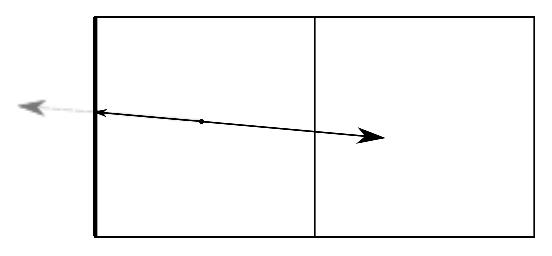
\includegraphics[width=12cm]{images/advection_clamping_borders}
\caption{Abschneiden der Geschwindigkeit an den Rändern}
\label{fig:stam_clamping_borders}
\end{figure}

Weiterhin muss auch der Fall, dass der zurückberechnete Vektor
$(i,j,k) - \Delta t \cdot u_{i,j,k}^t$ in einem Hindernis landet,
behandelt werden. Hierfür kann man einen Geschwindigkeitswert
von $(0,0,0)$ annehmen, was einem stationären Hindernis wie einem
Gebäude entspricht. Es ist aber auch möglich, ein weiteres Vektorfeld
$\vec{u}_{\PimiddyFormelText{boundary}}$ zu verwalten, in dem für jede
Gitterzelle die \emph{Geschwindigkeit} des dort vorhandenen
Hindernisses notiert ist. Dies wurde in~\cite{Crane2007}
umgesetzt. Für die Simulation in dieser Arbeit wurde von unbeweglichen
Hindernissen ausgegangen.

\subsection{Äußere Kräfte}

Die äußeren Kräfte werden in dem Term $g$ zusammengefasst und schlicht
auf die Geschwindigkeit addiert. In diesem Term lassen sich mehrere
interessante Effekte umsetzen, wie Auftrieb oder die Schwerkraft. In
diesem Abschnitt werden zwei dieser Effekte vorgestellt.

\subsubsection{Gravitation}

Zu den äußeren Kräften gehört die \emph{Gravitation}. Diese lässt sich
sehr einfach ausdrücken:

\begin{equation}
F_g = \Delta t (0,-9.81,0)
\end{equation}

\subsubsection{Wirbelstärkenerhaltung}

Der Advektionsschritt enthält eine lineare Interpolation, um die
Geschwindigkeitswerte in der Nachbarschaft des zurückverfolgten Partikels zu
finden. Diese simple Interpolationsmethode führt allerdings dazu, dass
Genauigkeit bei der Simulation verloren geht. Dadurch werden viele interessante
Phänomene in Fluiden, wie die starke Wirbelbildung bei Rauch, gedämpft und
treten nicht mehr so stark in Erscheinung.

Um dies auszugleichen, gibt es mehrere Ansätze. MacCormack hat ein
Advektionsverfahren entwickelt, was nicht mehr unbedingt stabil ist, aber eine
bessere Fehlerabschätzung liefert (\cite{Selle2008, Crane2007}). Dadurch
entstehen mehr Wirbelphänomene, allerdings bietet diese Methode keine
Möglichkeit, Einfluss auf die Wirbelstärke zu nehmen.

Daher wurde statt des MacCormack-Verfahrens eine Technik namens
\PimiddyBegriff{Wirbelstärkenerhaltung} (\PimiddyEnglisch{vorticity
confinement}) umgesetzt. Sie ist einfach zu implementieren, schnell
und erlaubt, die Stärke zu variieren. Entwickelt wurde sie, um die
komplexen Turbulenzen in der Umgebung von Helikoptern zu
modellieren (\cite{Steinhoff1994}).

Die Idee ist, Wirbel zu identifizieren und an den \PimiddyQuotes{richtigen}
Stellen zu verstärken. Dazu wird zuerst die Rotation des Geschwindigkeitsfeldes,
$\vec{R} = \PimiddyRot \vec{u}_{i,j,k}$, bestimmt. Der Betrag der Rotation,
$|\vec{R}|$, gibt an, wie stark die Wirbelbildung in einem Punkt ist. Der
\emph{Gradient} des Betrags, $\PimiddyGrad |\vec{R}|$, zeigt also
von Bereichen niedriger Wirbelstärke zu Bereichen hoher Wirbelstärke.

Um die Wirbel zu verstärken, bildet man eine Kraft, die senkrecht zum
(normalisierten) Gradienten und zur Rotation ist:

\begin{equation}
\label{eq:stam_vorticity_confinement}
\vec{F}_{\PimiddyFormelText{vorticity}}
=
\varepsilon \cdot
\left(
	\frac
	{
		\PimiddyGrad \vec{R}
	}
	{
		|\PimiddyGrad \vec{R}|
	}
	\times
	\vec{R}
\right)
\end{equation}

Die Konstante $\varepsilon$ gibt die Stärke der Kraft an.

\subsection{Projektion}
\label{sec:stam_projection}

\subsubsection{Einleitung}

Die bisher vorgestellten Al"-go"-rith"-men vernachlässigen die
Un"-komp"-ri"-mier"-bar"-keit des Flu"-ids, sondern behandeln einzig
die Impulsgleichung. Nach der Advektion und der Addition der äußeren
Kräfte kann die zweite Bedingung
\ref{eq:navier_stokes_incompressibility_condition} in den
Navier-Stokes-Gleichungen also verletzt sein, und die Simulation somit
nicht mehr physikalisch korrekt. Außerdem sind die Randbedingungen
eventuell verletzt worden. Beispielsweise wurde bei der Advektion
nicht beachtet, dass das Fluid um Hindernisse herumströmen sollte. Für
beide Fälle kommt der Druck $p$ als Korrekturterm ins Spiel. In diesem
Abschnitt wird $p$ näher erläutert und ein Algorithmus zu dessen
Bestimmung vorgestellt. Danach werden die Randbedingungen der
Simulation näher betrachtet.

Gegeben sei ein beliebiges Vektorfeld $\vec{u}$, zum Beispiel das
Geschwindigkeitsfeld nach der Advektion und nach Anwendung der äußeren
Kräfte. Da $\vec{u}$ nicht mehr quellenfrei ist, ist eine Funktion
$\PimiddyProjection$ gesucht, die $\vec{u}$ auf ein quellenfreies
Vektorfeld abbildet ($\PimiddyDiv \vec{u} = 0$). Hierzu
bedient man sich eines Ergebnisses aus der Vektoranalysis:

\begin{PimiddySatz}[Helmholtz-Zerlegung]
Sei $\vec{u}$ ein zweimal stetig differenzierbares Vektorfeld auf einem
beschränkten Definitionsbereich. Dann lässt $\vec{u}$ sich zerlegen in
ein \emph{quellenfreies} Vektorfeld $\vec{w}$ und den \emph{Gradienten}
eines Skalarfeldes $p$:

\begin{equation}
\label{eq:stam_helmholtz_equation}
\vec{u} = \vec{w} + \PimiddyGrad p
\end{equation}
\end{PimiddySatz}

\Cref{eq:stam_helmholtz_equation} soll nach $\vec{w}$ aufgelöst
werden, denn dieses Feld ist quellenfrei. Das Feld $p$ ist aber
ebenfalls eine Unbekannte in der Gleichung. Um die Gleichung
aufzulösen, wendet man die Divergenz auf beide Seiten der Gleichung an
und nutzt aus, dass der Operator \emph{linear} ist ($\PimiddyDiv
(\vec{u} + \vec{v}) = \PimiddyDiv \vec{u} + \PimiddyDiv \vec{v}$).
Als Ergebnis erhalten wir:
\begin{equation}
\label{eq:stam_poisson_equation}
\PimiddyDiv \vec{u} = \PimiddyLaplace p
\end{equation}
Hier wurde ausgenutzt, dass $\PimiddyDiv \vec{w} = 0$ gilt. Es
entsteht eine sogenannte \PimiddyBegriff{Poissongleichung}. Ihre
Lösung ist ein Standardproblem in der Physik, und im Folgenden wird
ein Verfahren vorgestellt, welches \cref{eq:stam_poisson_equation} nach
$p$ auflösen kann. Mit $p$ kann man dann durch Umstellen und Bildung
des Gradienten $\vec{w}$ bestimmen:
\begin{equation}
\vec{w} = \vec{u} - \PimiddyGrad p
\end{equation}
Darauf aufbauend kann man dann den Operator $\PimiddyProjection$ als
die Funktion, die ein Vektorfeld auf den quellenfreien Anteil der
Helmholtz-Zerlegung abbildet, definieren:
\begin{equation}
\PimiddyProjection \colon \PimiddyReell^n \to \PimiddyReell^n
\end{equation}
Diese Funktion wird in der Literatur auch oft
\PimiddyBegriff{Projektion} genannt. Führt man $\PimiddyProjection$ am
Ende des Verfahrens aus, erhält man ein unkomprimierbares Vektorfeld.

\subsubsection{Lösung des Poissonproblems}

Um das Vektorfeld quellenfrei zu machen, muss folgende allgemeine
Poissongleichung nach $p$ gelöst werden:
\begin{equation}
\PimiddyLaplace{p} = x,
\end{equation}
wobei $x$ ein Skalarfeld ist.

Es existieren zahlreiche Lösungsverfahren für solch eine
Gleichung. Bei der Auswahl des Verfahrens muss beachtet werden,
welches Verfahren sich gut auf der Grafikkarte umsetzen lässt und
möglichst schnell eine akzeptable Lösung liefert.

Es haben sich mehrere \PimiddyBegriff{Iterationsverfahren} als
günstig herausgestellt. Verfahren dieser Art beginnen mit einer initialen Lösung
(beispielsweise schlicht $p=0$) und nähern sich dann in jedem Iterationsschritt
weiter der eigentlichen Lösung an.

Betrachtet man große Felder, bieten sich
\PimiddyBegriff{Mehrgitterverfahren} an. Diese wurden bereits
erfolgreich auf GPUs angewendet (siehe~\cite{Bolz2002,
Matthias2006}). Sie sind allerdings untrivial zu implementieren, da
intern ein zweites Iterationsverfahren benötigt wird (der sogenannte
Restriktionsoperator), sowie Methoden zum hoch- und runterskalieren
von 3D-Feldern.

Simplere Iterationsverfahren, die auch in der Praxis schon auf die GPU
übertragen wurden, sind SOR (\cite{Saltvik2006}),
Gauss-Seidel-Re"-la"-xa"-ti"-on (\cite{Stam2003}) und das
Jacobiverfahren (\cite{Crane2007, Harris2008, Peschel2009}). Letzteres ist besonders einfach zu implementieren
und gleichzeitig hervorragend für die GPU geeignet. Es wurde daher für
die Implementierung verwendet und soll jetzt näher erläutert werden.

\subsubsection{Das Jacobiverfahren}

Um das Jacobi-Verfahren zu veranschaulichen, soll es zunächst im
Eindimensionalen erläutert werden. Wir betrachten also kein diskretes 3D-Gitter,
sondern eine endliche Teilmenge der ganzen Zahlen (die Gitterbreite $\Delta x$
ist also $1$). Der Laplaceoperator entspricht in diesem Fall der zweiten
Ableitung von $p$.

Für die exakte Lösung $p$ des Poissonproblems muss an jeder Stelle $i$ gelten:

\begin{equation}
\label{eq:stam_jacobi_onedimensional}
\frac{
	p_{i+1} -
	2 \cdot p_{i} +
	p_{i-1}
}
{
	{(\Delta x)}^2
}
=
x_i
\end{equation}

Löst man diese Gleichung nach $p_i$ auf und setzt $\Delta x = 1$ ein, erhält
man:

\begin{equation}
p_i
=
\frac{
	p_{j+1} +
	p_{j-1} -
	x_i
}
{
	2
}
\end{equation}

Der Wert $p_i$ definiert sich also durch seine direkten Nachbarn $p_{i-1},
p_{i+1}$, daher ist die Gleichung für sich genommen nicht aufzulösen.

Sei nun eine Anfangslösung $p^0$ gegeben, z.\,B.\ $p^0_i = 0$ für alle $i$.
Dann lässt sich eine neue, bessere Lösung bestimmen, indem man die Werte aus
$p^0$ als Näherungen für die Nachbarn in der exakten Lösung nimmt:

\begin{equation}
\label{eq:stam_jacobi_onedimensional_iterative_solution}
p_i^1
=
\frac{
	p_{j+1}^{0} + p_{j-1}^{0} - x_i
}
{
	2
}
\end{equation}

Im nächsten Iterationsschritt berechnet man dann $p_i^2$ mit Hilfe von $p_i^1$,
usw., bis man nahe genug an die exakte Lösung herangekommen ist. In der Praxis
sind mindestens 20 Iterationen nötig, da das Verfahren sehr langsam konvergiert.

Eine leichte Konvergenzverbesserung erreicht man, indem man die rechte Seite von
\cref{eq:stam_jacobi_onedimensional_iterative_solution} nicht direkt als neue
Lösung nimmt, sondern zwischen der bisherigen Lösung und der neue Lösung mit
einem Gewichtungsfaktor $\omega$ interpoliert:

\begin{align}
\overline{p}_i^{n+1}
&=
\frac{
	p_{j+1}^{n} + p_{j-1}^{n} - x_i
}
{
	2
} \\
p_i^{n+1}
&=
(1-\omega) \cdot p_i^n + \omega \cdot \overline{p}_i^{n+1}
\end{align}

Dieses Verfahren wird \PimiddyBegriff{gewichtete Jacobi-Iteration} genannt. In
der Praxis hat sich ein Faktor von $\omega=\frac{2}{3}$ als günstig erwiesen.

Das Verfahren lässt sich nun auf 3 Dimensionen (6 Nachbarn) verallgemeinern:
\begin{equation}
\label{eq:stam_jacobi_3d}
p_{i,j,k}^{n+1}
=
\frac{
	p_{i+1,j,k}^n +
	p_{i-1,j,k}^n +
	p_{i,j+1,k}^n +
	p_{i,j-1,k}^n +
	p_{i,j,k+1}^n +
	p_{i,j-1,k-1}^n -
	x_{i,j,k}^n
}
{
	6
}
\end{equation}

\subsubsection{Randbedingungen in Differentialgleichungen}
\label{sec:stam_boundaries}

Bei der Berechnung des Drucks müssen Randbedingungen beachtet
werden. Dies merkt man zum Beispiel daran, dass nicht jede Gitterzelle
6 Nachbarn hat, um die rechte Seite von \cref{eq:stam_jacobi_3d}
auszuwerten. Außerdem muss der Druck in Hinderniszellen so gewählt
werden, dass das Fluid nicht in das Hindernis eindringt, wenn man den
Druckgradienten im letzten Schritt des Verfahrens von der
Geschwindigkeit subtrahiert. Hier sollen die umsetzbaren
Randbedingungen besprochen werden.

Es gibt im Wesentlichen zwei Arten von Randbedingungen bei einer
Differentialgleichung (wie der Poissongleichung), zum einen die
\PimiddyBegriff{Di\-ri\-chlet-Rand\-be\-ding\-ung\-en} und zum anderen die
\PimiddyBegriff{Von-Neu\-mann-Rand\-be\-ding\-ung\-en}:

\begin{itemize}
\item
	Bei Dirichlet-Randbedingungen wird der \emph{Wert} des Feldes am Rand
	fest vorgeschrieben. Beispielsweise könnte man die Druckwerte, die über
	den Simulationsrand hinausgehen (z.\,B.\ $p_{-1,-1,-1}$), als $0$ annehmen.
	Dies ist gewissermaßen bei der Advektion geschehen, wo die
	Geschwindigkeit bei Hinderniszellen als $(0,0,0)$ angenommen wurde.
\item
	Bei Von Neumann-Randbedingungen schreibt man die \emph{Ableitung in
	Richtung der Normalen} an einem Punkt vor:

	\begin{equation}
	\frac{
		\partial \vec{u}
	}
	{
		\partial \vec{n}
	}(x)
	=
	f(x)
	\end{equation}

	Beispielsweise könnte man $f(x)=0$ wählen. Wie bereits in
	\cref{sec:mathematics_incompressibility_condition_section} erläutert
	bedeutet das, dass die Geschwindigkeitspfeile nicht in ein Hindernis
	hinein- oder hinauszeigen dürfen, das Fluid selber darf sich aber tangential
	frei bewegen. Diese Randbedingung wird deshalb auch spezieller als
	\PimiddyBegriff{free-slip}-Randbedingung bezeichnet.
\end{itemize}

\begin{figure}[ht]
\centering
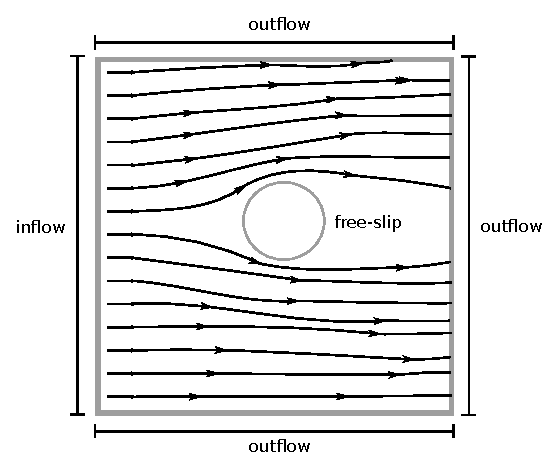
\includegraphics[width=12cm]{images/boundary_types}
\caption{Strömungslinien einer Beispielsimulation mit 3 verschiedenen Randbedingungen.}
\label{fig:stam_boundary_types}
\end{figure}

In der Simulation soll ein Teilbereich der echten Welt simuliert werden. Der
Wind wird von einigen Seiten künstlich in die Simulation gespeist. Dies nennt
man \PimiddyBegriff{inflow boundary} und ist eine Form der
Dirichlet-Randbedingung. Aus den verbleibenden Seiten soll der Wind frei aus der
Simulation \PimiddyQuotes{herausfließen}, als würde der Simulationsbereich dort
noch weitergeführt werden. Diese Art der Randbedingung nennt man
\PimiddyBegriff{outflow boundary}.

Simuliert man Rauch oder Wasser gibt es noch weitere Arten von
Randbedingungen.  Die Grenze zwischen Wasseroberfläche und Luft nennt
man \PimiddyBegriff{free surface}-Randbedingung. Um diese umzusetzen
müsste man außerhalb des Wassers $p=0$ setzen. Diese Randbedingung
wird hier nicht weiter beachtet.

Eine Zusammenfassung aller Randbedingungen ist in \cref{fig:stam_boundary_types} zu sehen.

\subsubsection{Randbedingungen in der Simulation}

Es werden zuerst die Randbedingungen für die Hindernisse betrachtet. Hier sollen
\emph{free-slip}-Bedingungen erzwungen werden. Diese soll nicht explizit
hergeleitet werden, es werden nur die Veränderungen am Jacobiverfahren
beschrieben.

Im bisher beschriebenen Jacobiverfahren betrachtet man jede Zelle $p_{i,j,k}$
des Gitters und bildet die Summe über alle Nachbarzellen. Um die Randbedingungen
einfließen zu lassen, testet man, ob die Nachbarzelle von einem Hindernis
ausgefüllt ist (hier benutzen wir das Hindernisfeld $b_{i,j,k}$, welches eingangs
beschrieben wurde). Gehört die Zelle zu einem Hindernis, wird nicht der
Druckwert der \emph{Nachbarzelle} zur Summe addiert, sondern der Wert der
\emph{aktuellen Zelle} (siehe \cref{fig:stam_modified_jacobi_algorithm}). Auf
diese Weise kommt es zu keinem Druckunterschied in Richtung eines Hindernisses,
der Gradient in dieser Richtung ist also
0. \cref{alg:stam_modified_jacobi_algorithm} zeigt den modifizierten
Jacobi-Algorithmus.

\begin{algorithm}
\caption{Der modifizierte Jacobi-Algorithmus}
\begin{algorithmic}
\Function{jacobi}{$p,x$}
	\State $p' = 0$
	\Comment{Ergebnisfeld ist $p'$}
	\ForAll{$(i,j,k)$}
		\State $\textrm{sum } \gets 0$
		\ForAll{Nachbarn $(i',j',k')$ von $p_{i,j,k}$}
			\If{$b_{i',j',k'} = 1$}
				\State $\textrm{sum} \gets \textrm{sum} + p_{i,j,k}$
			\Else
				\State $\textrm{sum} \gets \textrm{sum} + p_{i',j',k'}$
			\EndIf
		\EndFor
		\State $\textrm{new} = (\textrm{sum} - x_{i,j,k})/6$
		\State $p_{i,j,k}' \gets (1-\omega) \cdot p_{i,j,k} + \omega \cdot sum$
		\Comment{Gewichtete Jacobi-Iteration}
	\EndFor
	\State \Return $p'$
\EndFunction
\end{algorithmic}
\label{alg:stam_modified_jacobi_algorithm}
\end{algorithm}

\begin{figure}[ht]
\centering
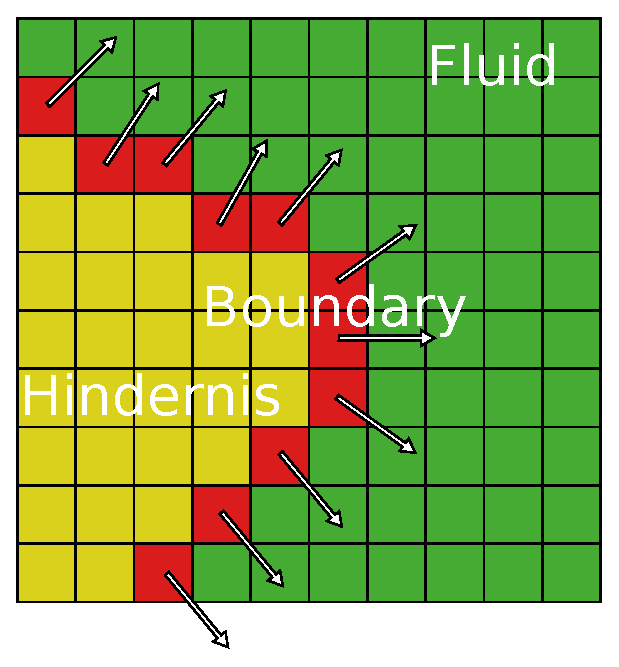
\includegraphics[width=9cm]{images/boundary_with_normals}
\caption{Hindernisse mit zugehöriger Normale}
\label{fig:stam_boundary_with_normals}
\end{figure}

Der Jacobi-Algorithmus löst die Poissongleichung allerdings nur annähernd.
Folglich werden auch die Randbedingungen nur annähernd gelöst. Dies kann im
nächsten Simulationsschritt zu Problemen führen. Daher wird in der
Implementierung die free-slip-Rand\-be\-din\-gung nach dem Projektionsschritt
erzwungen (also nachdem der Gradient des Drucks vom Geschwindigkeitsfeld
subtrahiert wurde).

Idealerweise bräuchten wir dazu noch ein Feld $\vec{n}_{i,j,k}$, was in jedem
Punkt die Normale des Hindernisses angibt (siehe
\cref{fig:stam_boundary_with_normals}). Dies wurde in einigen
Arbeiten umgesetzt (\PimiddyzB{} \cite{Bordignon}), es gibt jedoch eine Vereinfachung,
die dieses Feld nicht benötigt: Man iteriert erneut über alle
Gitterzellen und testet für jede Gitterzelle $(i,j,k)$, welche
Nachbarzellen von einem Hindernis ausgefüllt sind. Die zugehörige
Komponente der Geschwindigkeit $\vec{u}_{i,j,k}$ wird dann auf 0
gesetzt (siehe \cref{alg:stam_enforce_free_slip}).

Für die outflow-Randbedingungen am Simulationsrand wird jede Randseite der
Simulation einzeln betrachtet. Die Geschwindigkeit einer Randzelle wird ersetzt
durch die Geschwindigkeit der \PimiddyQuotes{nächst inneren} Zelle.
Beispielsweise werden die Geschwindigkeitswerte $\vec{u}_{0,j,k}$ (also die an
der linken Simulationsseite) ersetzt durch die Werte $\vec{u}_{1,j,k}$. Analoges
wird für die anderen Seiten des Kubus getan, mit Ausnahme dort, wo
inflow-Randbedingungen bestehen, wo also Wind in die Simulation hineinfließt.
Dadurch ergibt sich am Rand die Divergenz 0, der Druck ist hier also auch
annähernd 0.

\begin{figure}[ht]
	\begin{subfigure}[t]{0.5\textwidth}
		\centering
		\includegraphics[width=\textwidth]{images/boundary_field_for_pressure}
		\caption{Ein beispielhaftes Hindernisfeld $b_{i,j}$}
	\end{subfigure}
    ~
	\begin{subfigure}[t]{0.5\textwidth}
		\centering
		\def\svgwidth{\textwidth}
		\input{images/pressure_boundary.eps_tex}
		\caption{Die in die Druckberechnungen einfließenden Werte.}
\label{fig:stam_modified_jacobi_algorithm}
	\end{subfigure}
    \caption{Druck in Zusammenhang mit Hindernisfeldern}
\end{figure}

\begin{algorithm}
\caption{Die abschließende Erzwingung der Randbedingungen}
\begin{algorithmic}
\Function{FreeSlipBoundary}{$\vec{v},b$}
	\ForAll{$(i,j,k)$}
		\If{$b_{i-1,j,k} = 1$ or $b_{i+1,j,k} = 1$}
			\State $\vec{u}_{i,j,k}^x = 0$
		\EndIf
		\If{$b_{i,j-1,k} = 1$ or $b_{i,j+1,k} = 1$}
			\State $\vec{u}_{i,j,k}^y = 0$
		\EndIf
		\If{$b_{i,j,k+1} = 1$ or $b_{i,j,k-1} = 1$}
			\State $\vec{u}_{i,j,k}^z = 0$
		\EndIf
	\EndFor
\EndFunction
\end{algorithmic}
\label{alg:stam_enforce_free_slip}
\end{algorithm}
